
\section{Multi-omics} \label{s:multi-omics}

% introduction the importance of genetics as a field (when was born), key discoveries
% The field of genetics is moving rapidly since 1953 when Francis Crick and James Watson discovered the structure of the DNA; a breakthrough built on the work of Rosalind Franklin \& her lab. Subsequent work in the field highlighted the central role that genes play in all living organisms and it represented the missing piece in Darwin's theory of evolution. 

To understand cancer, we need to know how the cells work and replicate in the tissues, which is only possible by studying the constituent blocks that are represented or regulated by proteins, which in turn are created by the instructions from DNA. To find the faulty biological processes the analysis needs to be performed on both the tumorous and healthy cells/tissue enabling the comparison between normal and abnormal behaviour. To do this, scientists use multiple streams of information from molecular biology like gene expression (transcriptomics), mutations (genomics), lipidomics, proteomics etc. Through this existing biological data combined with modelling, researchers are creating linkings such as gene network interactions. 

% I would put in brackets after each type the omics technology which generates it: gene expression (transcriptomics), mutations (genomics), proteomics, lipidomics, metabolomics etc., and then say that existing biological data and modelling approaches can be used to create links, such as gene network interactions


% Technicality. It's only multi-omics if you use more than one type to answer a single problem. The broader technologies are called "omics". You could say: "This project focuses on combining multiple information streams into a single multi-omics approach...."

% introduction to DNA & RNA, the genetic diversity on Earth, why it's important and some fascinating facts
A useful analogy for engineers is that a DNA molecule is the equivalent of a hard drive where information is stored, while the RNA is similar to RAM. This represents the relevant information (from the DNA) needed to make new copies of a particular protein. Even though all the living organisms share a large amount of DNA, each species has its features\footnote{Interestingly the same mechanism to build proteins is present in animals, plants and is highly similar in bacteria and other living organisms.}. Across a species, the genetic material varies slightly making the individual both unique and common, depending on the reference point. Interestingly, when at birth the cells of an individual share the same genetic information, but as it ages the new cells created will start to have anomalies specific to tissue. Cancerous tissue has an uncommonly large number of these changes.

\begin{figure}[!ht]
  \centering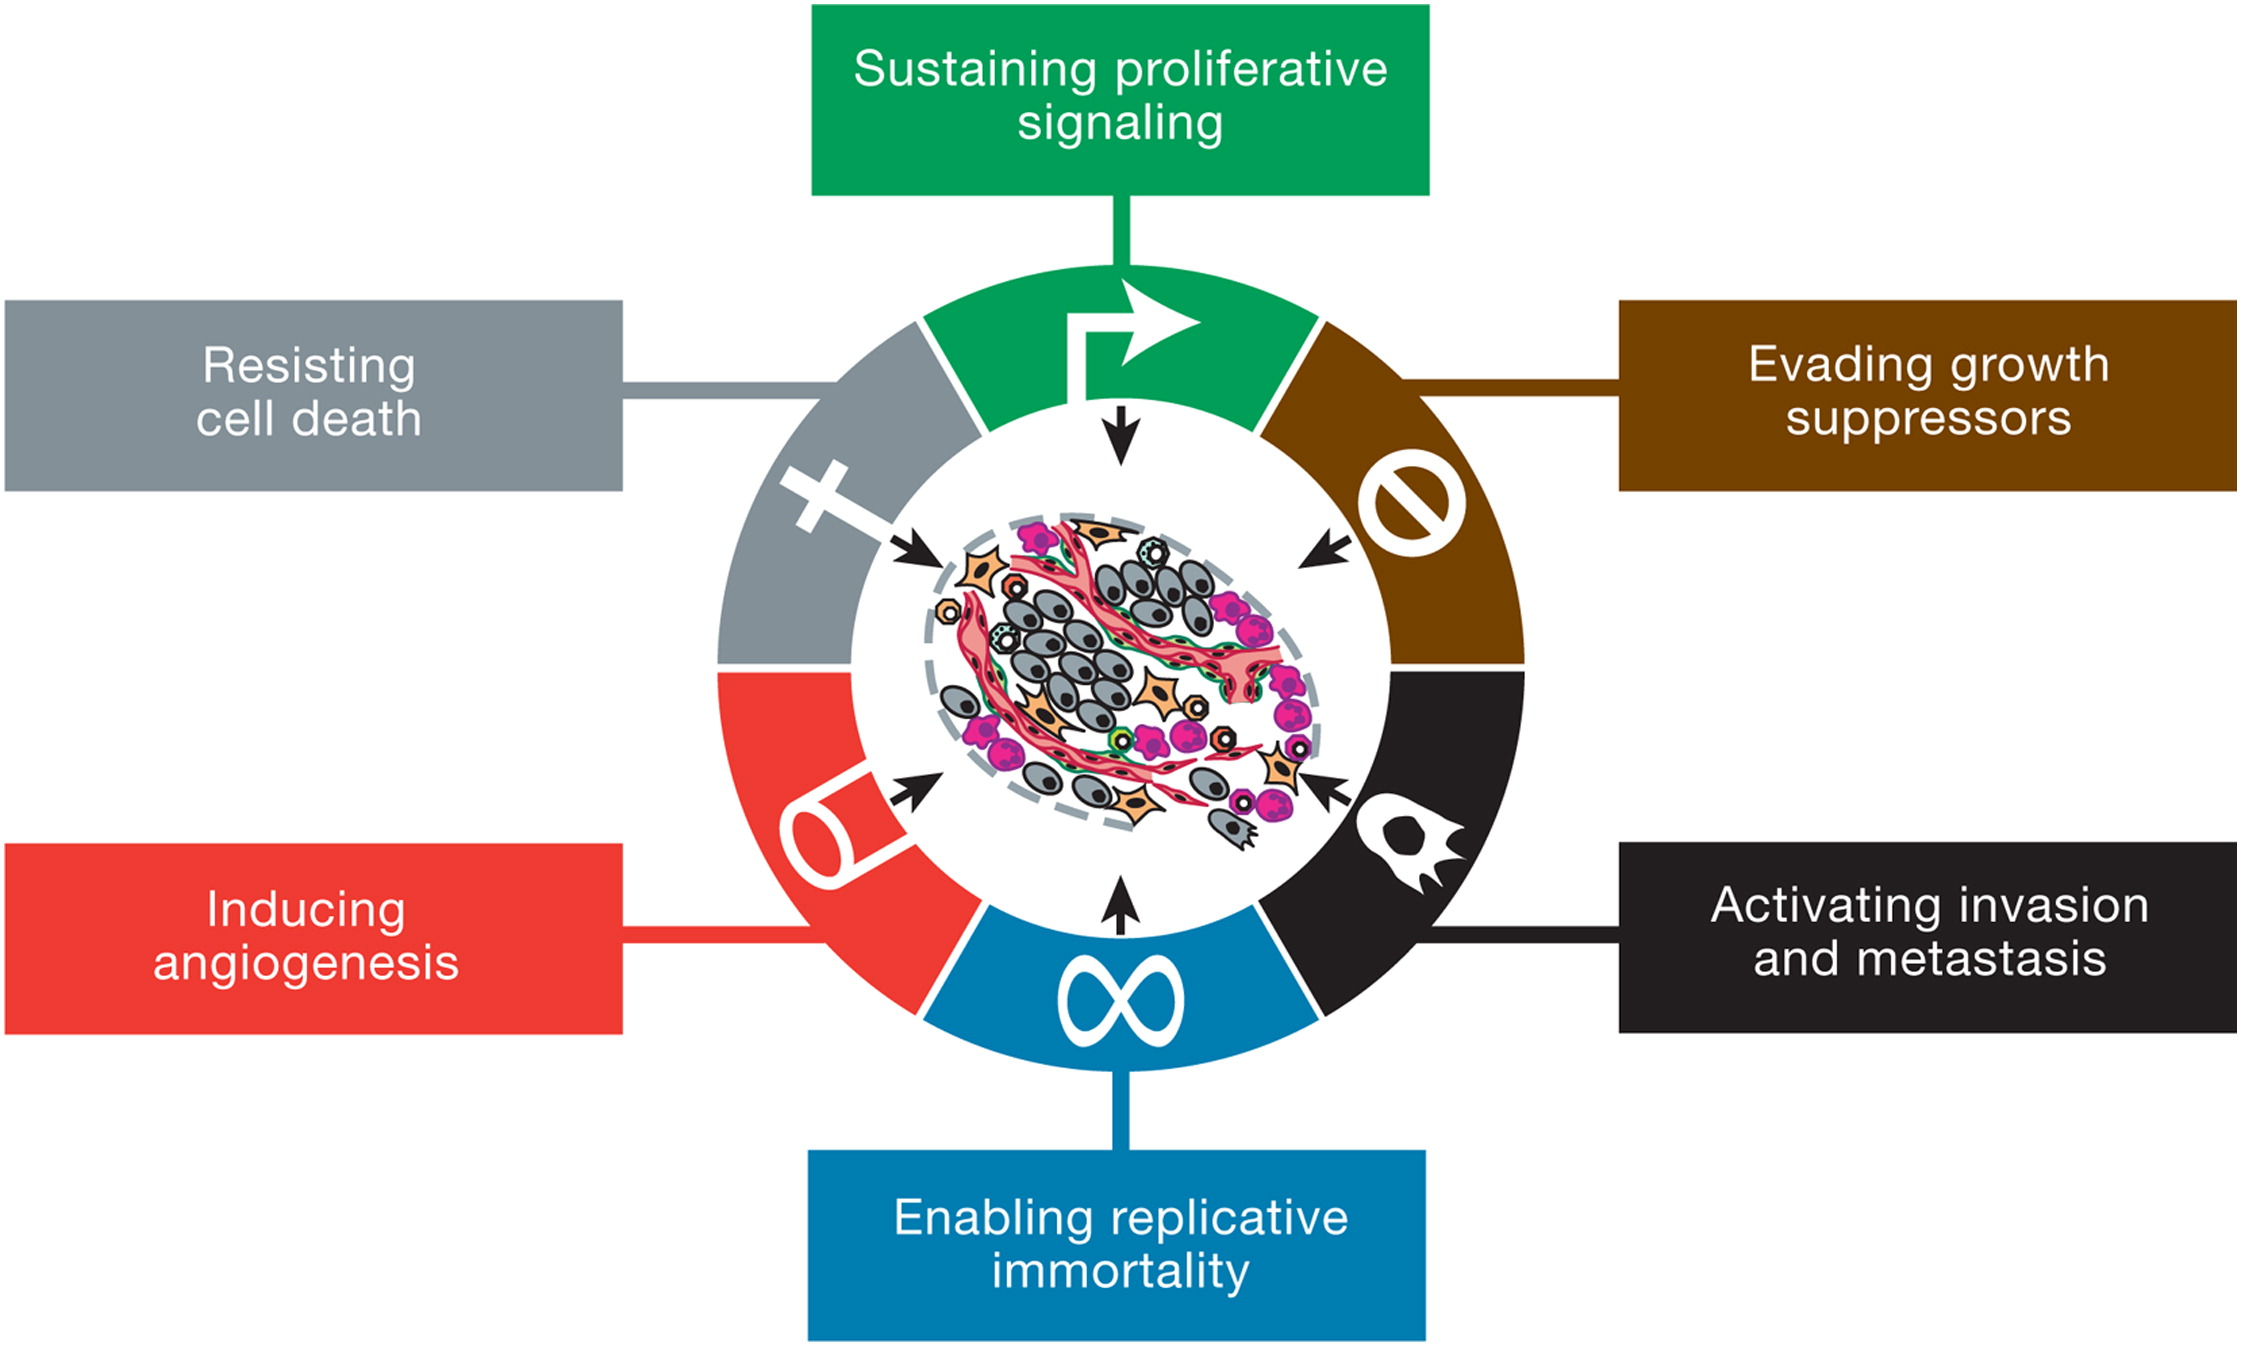
\includegraphics[width=0.8\textwidth,height=0.8\textheight,keepaspectratio]{Images/TCGA/tumour_causes}
    \caption{Hallmarks for the cancer tumours\cite{Hanahan2011-px}. The Sustaining proliferative signalling feature means that the cancerous cell will be 'encouraged' to divide while evading the growth suppressors and resist cell death will only aid the birth of new malign cells. On top of that, these cells have the replicative immortality trait. Activating invasion and metastasis means that the cells are capable of spreading to other parts of the body. Lastly, angiogenesis refers to the tumours capability to draw nutrients to sustain itself through the creation of blood vessels. }
    \label{fig:hallmarks_cancer}
\end{figure}

% Small paragraph showing the ideas
Numerous sources are causing genetic alterations in a healthy organism which can lead to diseases. From Figure \ref{fig:hallmarks_cancer} it can be seen that a large proportion of the tumour hallmarks are related to the cell division cycle that is because of all the properties of a cell, this is the one that comes under most natural selection because it leads to growth/expansion of the tumour. From Evading growth suppressors to resisting cell death, the cancerous cell will not stop dividing and will slowly conquer the tissue as the healthy cells will reach the end of their cycle and die.

A driving motivation in cancer research is to learn the gene mechanisms to develop a cure for the disease. Medicine made important progress in cancer research \& diagnosis but cancer remains an unsolved problem. One of the reasons for this is the intricate mechanism of gene interactions that due to its complexity is difficult to understand. On top of that, we cannot collect the ideal data\footnote{The ideal genomic dataset is represented by a large number of tumour samples, matched with a blood sample, and multi-omic sequenced (proteins, RNA, mutations etc.). Multiple samples from the same donor to track genetic changes as the disease progress and map it to the appropriated genes.)} to make accurate predictions; imagine a person suffering from cancer and scientists constantly asking for more data (i.e. biopsy). Thus, due to both ethical and clinical considerations, samples are typically taken at the point of cancer surgery, so repeat samples are often unfeasible. Therefore, it is challenging to determine the exact gene interactions which drive a subtype of cancer and as a matter of fact, any disease. 

% also, due to both ethical and clinical considerations, samples are typically taken at the point of cancer surgery, so repeat samples are often unfeasible" - or something

% introducing the datasets and the efforts to get data that may be useful for us. This includes:
%  expression, mutation and signalling 
Sequencing techniques are becoming more affordable every year, and now companies like 10X Genomics can extract information about the gene expression at the level of a single cell. In addition, we get mutation data with base-pair precision; i.e. we know which part of the gene sequence presents an anomaly. Even with the costs lowering every year, sequencing large cohorts is expensive, and there are just a few large studies. One of the largest is \acrshort{tcga}\cite{Tcga2018-sj} which consists of roughly 20000 samples across 33 cancer types. An impressive effort, but if one focuses on particular cancer, the available data is drastically lower. For example, the data available for \acrfull{mibc} cancer is 408 samples with both expressions and mutation information\cite{Robertson2017-mg}.  

% present some of the characteristics of the data: small samples, high dimensionality and briefly present some of the methods presented
This becomes a problem of the low sample set and large features (there are more than 56k genes in a sample), which is usually the other way in the problems addressed in typical ML problems. An engineer may fall into the trap that this challenge is solvable by the dimension reduction techniques with established algorithms like \acrfull{pca}, \acrfull{umap} or \acrfull{tsne}. Followed up by applying a clustering algorithm like k-means, Ward, Birch etc. . This is the approach used in all datasets which were recently combined in the muscle-invasive bladder cancer consensus \citet{Kamoun2020-tj}.

% Problems if we just use dim reductions or if we don't take into consideration all aspects of the genes
However, this suffers from a major assumption given by the dimension reduction algorithms that tend to select the data points with the highest variance. From an information theory stance, this is true as the relevant information is given by high variance\footnote{That is, the more different a data point is from the average, the more information contains. One can think about this as, if you were to live in the UK, you were more interested when the sunny days are, not when it rains.}. However, a gene that is a common driver for cancer disease will have a high median/average but not a high variance. For example, TP53 is a cell cycle checkpoint control that checks the DNA integrity before allowing a cell to commit to cell division, and when the gene is mutated indicates that the cell cycle is not under the control. While exploring the TCGA data for bladder cancer \cite{Tcga2018-sj,Robertson2017-mg} it was observed that the expression for this gene has a consistent value across the sample, hence a low variance. An explanation for this might that the TP53 is commonly mutated across the bladder cancer as seen in Figure \ref{fig:2020_consens} from the next section. Such instances impose a great challenge as the model needs to avoid dismissing genes that don't have a large variance.

% Later, we will see that this can be measure by the exclusive is the mutations/expression related to the other genes in the set.

The previous work done in the field can be categorised based on the data given to the models. This can vary from focusing on how mutations affect the genes pathways, the effect of transcriptomics or processing the signalling pathways. This represents the foundation for multi-modal or in bioinformatics terminology, multi-omics approaches where the hypothesis is different types of data yields better predictions. This project focuses on combining multiple information streams into a single multi-omics approach. The hypothesis is that mutations (covered in \ref{s:mutations}) affect gene expression (\ref{s:rnaSeq}) and considering both will yield a better subtyping of the \acrlong{mibc}.

\subsection{Gene expression data} \label{s:rnaSeq}

\vspace{3mm}
% \noindent\rule{17cm}{0.2pt}
\fbox {
    \parbox{\linewidth}{
      \begin{itemize}
        \item Focus on subtyping the cancer based on RNAseq
        \item Six consensus classifications for bladder cancer by \citet{Kamoun2020-tj}
        \item Prevalent approch is hierarchical clustering on RNAseq data
        \item TCGA classification by \citet{Robertson2017-mg}
        \item SNN were used in microarray data
      \end{itemize}
    }
}
\vspace{3mm}

% Talk about how and why unsupervised learning is used for RNAseq.
% Talk about the consensus in the 2020 paper
The proteins are the building blocks of every living organism and implicitly of the tissues. To understand the malfunctioning of the biological processes causing cancer, protein data (proteomics) are the ideal data to analyse malignant behaviour. However, measuring proteins in samples is hard and expensive, and as an alternative, RNAseq data is used which is also increasing more affordable. It is worth mentioning that this measures the abundance (or the transcript) of a gene\footnote{Remember the analogy of the RAN at the start of this Chapter. The DNA is the instruction from hard drive, where the RNA is the instruction from memory and the protein is what the instruction creates.} which is a proxy for the proteins produced, consequently, it's not a direct measure of the proteins it might have biological limitations. From an engineering perspective, any additional step in the process is a potential risk to add more errors to the output. Similarly, the RNAseq may not always represent an accurate representation of the biological processes. This can be overcome by domain knowledge in the field, and it is where collaboration with JBU plays a vital role.

Genomics datasets (including RNAseq) are characterised by having a small number of data points (tissue samples) but a large number of features (number of genes). Another aspect of the available datasets is that the samples usually come from tumours because obtaining a sample involves surgery, hence there is less publicly available data on healthy tissue. In contrast, as JBU's focuses on bladder tissue there is data collected on the urothelium which is the normal tissue counterpart of the cell that is usually transformed in urothelial cancer.

% specifically the urothelium which is the normal tissue counterpart of the cell that is usually transformed in urothelial cancer
Cancer is not one disease and There has been a lot of effort in subtyping the cancers as defining subgroups will help to diagnose and treat patients. In the 2020 paper \citet{Kamoun2020-tj} combine six approaches \cite{Mo2018-rl, Damrauer2014-tc, Choi2014-ed, Marzouka2018-ge, Rebouissou2014-ep,Robertson2017-mg} on bladder cancer subtyping to find a consensus in subgrouping. This resulted in 6 subtypes which can be seen in Figure \ref{fig:2020_consens} with their characteristics. It can be noticed that some subtypes are more prevalent than others, with Luminal Papillary (24\%) and Basal/Squamous (35\%) being most common, followed by Luminal Unstable and Stoma Rich (both 15\%). Moreover, each subtype has a different mutations signature only enforcing the project hypothesis by adding mutation to the RNAseq data will yield better cancer classifications.

\begin{figure}[!htb]                                  
    \centering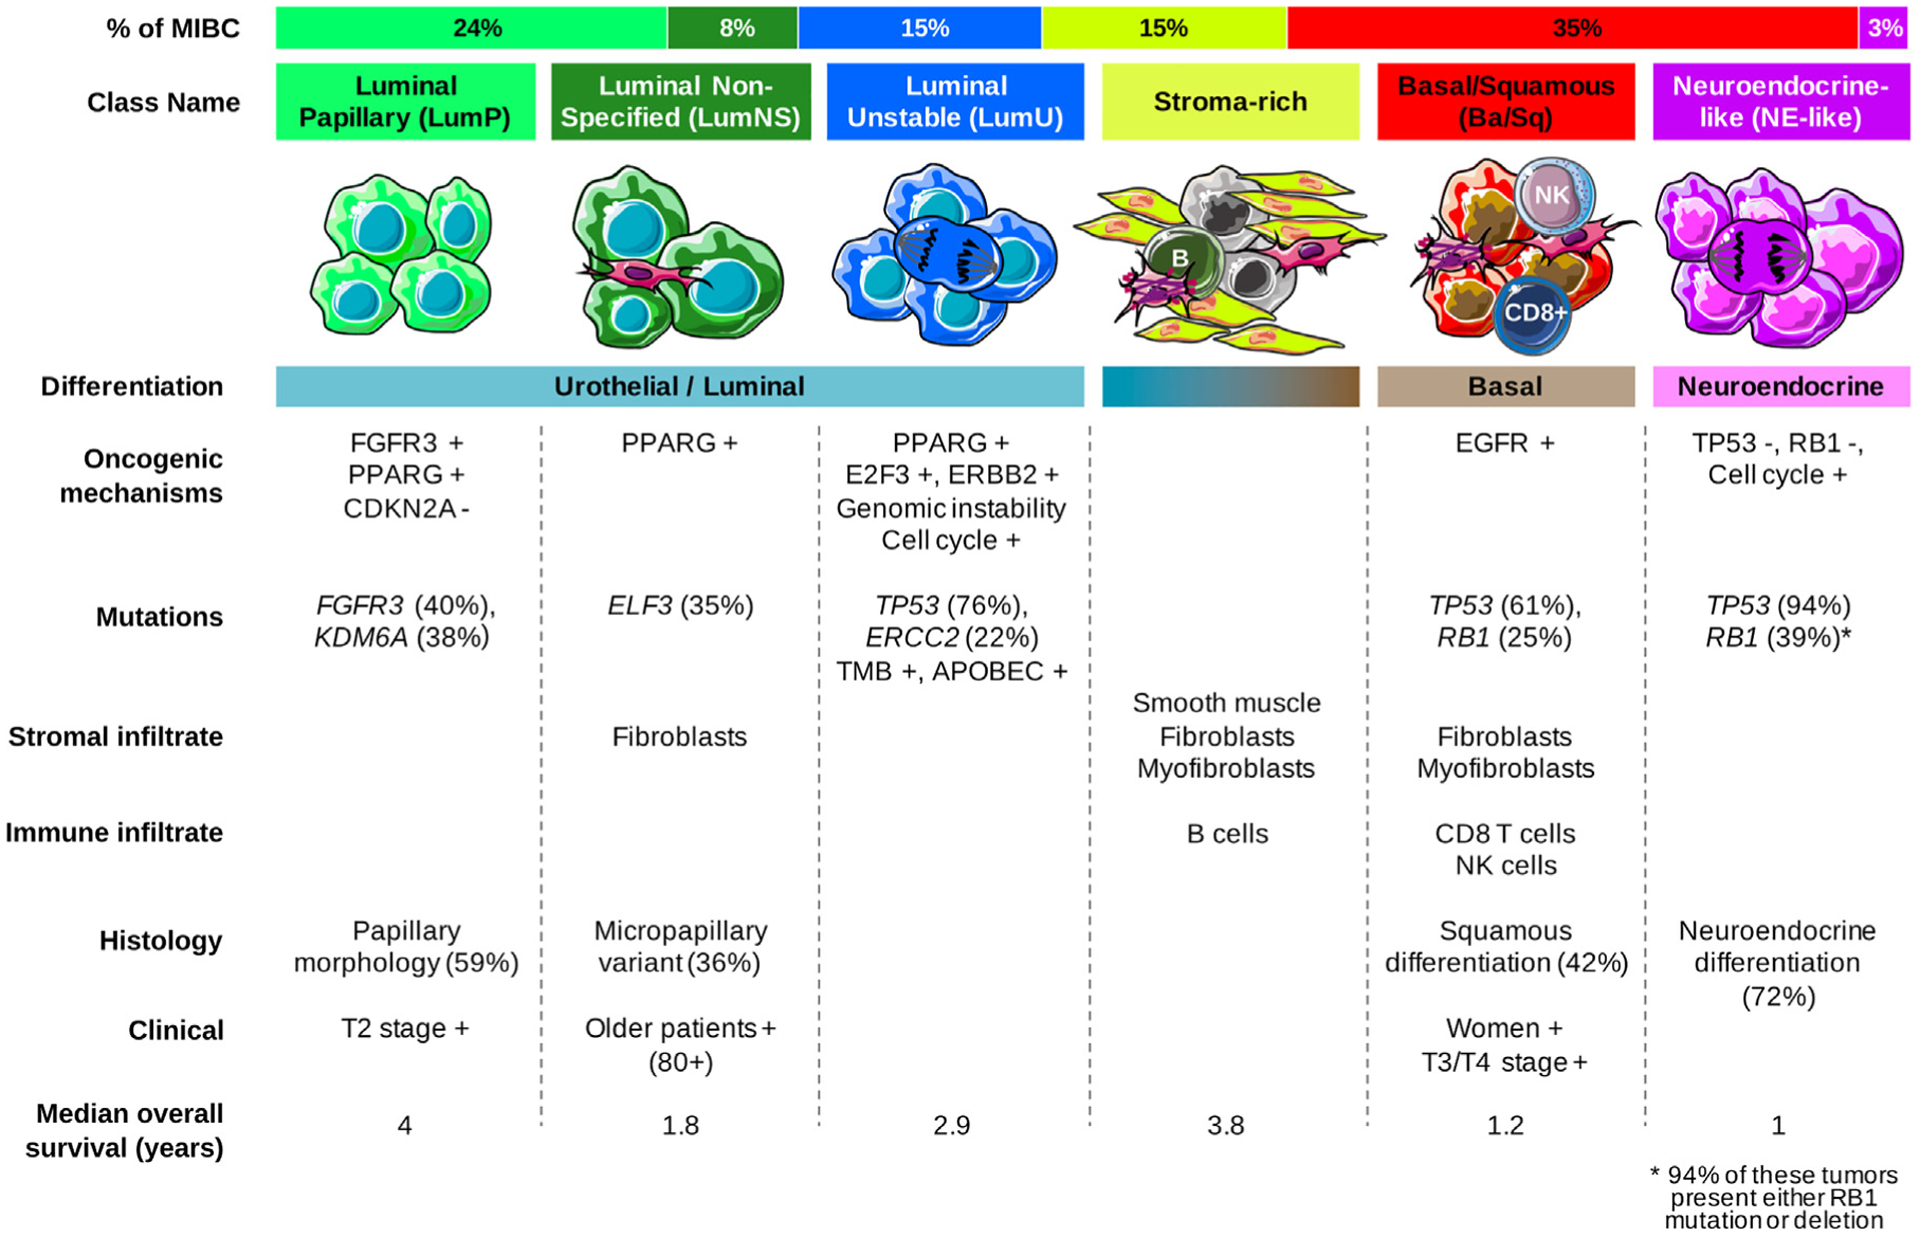
\includegraphics[width=1.0\textwidth,height=1.0\textheight,keepaspectratio]{Images/TCGA/2020_consensus_subtypes.jpg}
      \caption{The six different subtypes of \acrfull{mibc} by the consensus classifier\cite{Kamoun2020-tj}, the names are based on their differentiation status, morphology etc. There are three different types of Luminal Bladder cancer: most common being the ones related to papillary morphology (LumP), Luminal Non-Specified (LumNS) showing immune markers, and Luminal Unstable (LumU) is the newest luminal subtype. Basal/Squamous (Ba/Sq) is the most common bladder cancer and is related to the Squamous tissue. Neuroendocrine-like (NE-like) share similarities with Ba/Sq cancer and Stroma-rich are likely not to be a biological group but a collection of samples that contain artefacts from the collection or/and other intermediate processes. Imaged adapted from \cite{Kamoun2020-tj}.
      }
      \label{fig:2020_consens}
  \end{figure}
  \FloatBarrier

There are few points worth emphasising in the consensus paper, first, all the approaches\cite{Mo2018-rl, Damrauer2014-tc, Choi2014-ed, Marzouka2018-ge, Rebouissou2014-ep,Robertson2017-mg} considered were using hierarchical clustering. Secondly, all models are given only RNAseq data\footnote{Robertson et al. use domain knowledge to choose the number of subtypes.} and the studies are not using the same data (except \cite{Robertson2017-mg, Mo2018-rl} which both are using TCGA data). One consequence of using different data sources is that each study proposed a different set of subgroups. To reach the consensus on subtyping, \citet{Kamoun2020-tj} combined all the datasets resulting in 1750 samples and run the models enlisted above. All the output from the approaches enlisted were analysed together as a network and based on this the six consensus subtypes were defined in Figure \ref{fig:2020_consens}.

% you don't need to get too much into biology. In a couple of lines you can say why groups were named - papillary from papillary morphology (google it), Ba/Sq and neuro from markers indicative of those tissue differentiation states (so we know markers for them). You don't need to list subgroup x is called this because... but say that subgroups are named based on their differentiation status, morphology etc. Stroma-rich, not a "proper" biological grouping (most likely) etc etc


% Talk about the consensus in Robertson paper
One of the approaches considered in the Consensus was the work done by \citet{Robertson2017-mg} which found five bladder cancer subtypes in TCGA dataset. The main difference between the two classifications consists in that Luminal-infiltrated (TCGA subtype) was reclassified as Stroma-rich and \citet{Robertson2017-mg} does not classify Luminal unstable (LumU). The TCGA dataset consists of 408 different donor bladder samples with  $\sim$56k expressed genes each. At the pre-processing stage, the under-expressed genes were removed, and only the 25\% with the highest standard deviation were selected, reducing the number of genes to 3347. The authors used Agglomerative Hierarchical clustering with average linkage and found five clusters. This was supported by another approach Bayesian \acrfull{nmf} \cite{Schmidt2009-zh}.

 
% Talk about sci-fold
More recent work is \citet{Tian2021-vu} who used the Stiefel manifold method on gene expression, miRNA expression data and DNA methylation. Compared to previous work discussed in this subsection, Tian et al. are focusing on four other cancers from TCGA dataset: glioblastoma multiforme (GBM), breast invasive carcinoma (BIC) Skim Cutaneous Melanoma (SKCM) and Acute Myeloid Leukemia (AMIL). In their work, the authors suggest that using both gene expression and DNA methylation would yield better subtyping but they do not provide clear results on their model.

% other approaches 
The microarrays data is an older method to obtain genomic information from tissue and compared to RNAseq is more error-prone. Some studies take multiple measures of the biopsy which adds a time dimension to the data, making it a good fit for Spiking Neural Networks. In their recent work, \citet{Capecci2020-uj} combine SNN with EA to process microarrays data to classify the gene interactions based on their temporal feature. As the collected samples from human skin with dermatitis which is not cancer/tumour, the data used did not include any mutation information. Despite that, their work may facilitate our research through their encoding mechanism or pre-processing techniques used.

% Introducing neuroevolution
This is not the only use of microarrays data, \citet{Grisci2019-xn} have introduced a neuroevolution model for analysing microarrays. Their research is built on the FS-NEAT\cite{Whiteson2005-dn} which is an idiosyncratic version of the NEAT model (neural Networks through Augmenting Topologies)\cite{Stanley2002-tg} focused on the feature selection (FS). As the name suggests NEAT\cite{Stanley2002-tg} uses evolutionary methods to find the optimal network structure (i.e. topology) of \acrshort{ann} which at the time of the paper was a novel approach\footnote{Previously evolutionary and connectionists approaches were combined only to derive the initial weights of the ANNs.}. The work done by Grisci et al. is worth considering for their unusual application of neuroevolution to the genomic data. Nevertheless, their dataset is different from the gene expression data available on TCGA as the data used by \citet{Grisci2019-xn} contained observations from the same sample at different times.

% Also, you can infer some mutations from RNA sequencing (but not accurate for several reasons), but microarray is intensity only, you never get a sequence to say what a mutation is. Doing double/treble/quadruple etc work on the same sample is v. expensive and RNAseq is the cheapest one. This all plays into why it is used so much, but it's chicken and the egg in a lot of ways.

% skin with dermatitis is not cancer/tumour so no they wouldn't include mutational data - it is an inflammatory (allergic) condition

\subsection{Gene Mutations} \label{s:mutations}

\vspace{3mm}
\fbox {
    \parbox{\linewidth}{
      \begin{itemize}
        \item Models focused on finding mutated genes
        \item Indentifying the driver genes is formalised as finding a submatrix of relevant genes 
        \item Dendrix (\citet{Vandin2012-cf}) is a popular model with several variations
        \item MDPFinder (\citet{Zhao2012-wj}) uses EA to find the submatrix of relevant genes
      \end{itemize}
    }
}
\vspace{3mm}


Gene mutations are anomalies that occur at the gene level within the DNA, where one (or more) blocks (nucleotides) are replaced by the other bases (3 possibilities) or insertion/deletion can happen to the gene. Depending on where they occur in the gene sequence, the mutations have a less or worst negative effect on protein production. This means that simply knowing that a gene is mutated or not, is not enough to correlate to an ill behaviour but we need information about where the gene happened. The mutations that contribute to tumorigenesis are called driver genes and the ones who have a neutral contribution are known as passenger mutations\cite{Ciriello2012-hi}. To retrieve the mutated genes Whole Exome Sequencing (WES) technique is used which targets portions in the gene (exome - more likely to be relevant and cost-effective) and compare it with the reference genome\cite{Schneider2016-ml}. This section covers computational models that seek to find the driver gene in a tissue whereas the project aims to improve bladder cancer classification using mutation data. Despite the two having different aims, the methods should be relevant for the project.

%  dimension reduction, gene subsets, finding the submatrix 
  \citet{Vandin2012-cf} determined gene mutation exclusivity by variables and demonstrated that finding the subset (or submatrix) is an NP-hard problem\footnote{ NP stands for Non-deterministic polynomial time and computer scientists describe the NP problem as the most complex problems in terms of the computational cost.}. Thus, the selection process of the relevant genes has been demonstrated by the authors to be NP-hard, meaning that it takes a lot of computational resources to solve it due to its complexity.
   Dendrix, the introduced model, is constructing a submatrix with the driver genes of the disease from a larger set of genes. Specifically, it looks at finding the mutated genes that have the following two properties: high coverage (common) and high exclusivity (specific to some samples). The genes that need to be included in the submatrix are chosen by a weighting factor, which takes into account the above two properties. Dendrix comes with two solutions: a greedy algorithm (requires a large dataset) and a stochastic one, Monte Carlo. Importantly, Dendrix is a \textit{de novo} algorithm that does not need \textit{a priori} data regarding the gene interactions to determine their significance.

% Introducing Comet 
Building on the work of \citet{Vandin2012-cf} there are several variations of the Dendrix model proposed \cite{Leiserson2013-da,Szczurek2014-dh,Leiserson2015-yk}. Noteworthy is the COMET (\citet{Leiserson2015-yk}) model developed in collaboration with Vandin to overcome the bias introduced by the highly mutated genes to the computational models derived from Dendrix \cite{Vandin2012-ns}. \citet{Leiserson2015-yk} accomplished this by introducing a scoring mechanism that measures how exclusive a mutation is to cancer. This is more advanced of the weighting function from the original paper by Vandin et al. which was used to search for the submatrix of the driver genes. They compared the results with different models\footnote{Multi-Dendrix\cite{Leiserson2013-da} created by the same group and is a variation of the Dendrix (\citet{Vandin2012-cf} model). The other model that they compare with is mutex\cite{Babur2015-qk} which is also looking at the exclusivity of the mutations.} using datasets from TCGA and the COMET outperforms all the other models\cite{Leiserson2013-da,Szczurek2014-dh} in finding the genes predominantly mutated in particular cancer. Another characteristic of this model is that it doesn’t need a large dataset which makes COMET a veritable model for processing mutations information.

% Introducing MDPFinder 
%  The novelty of Zhao et al. is that they take the problem defined by Vadin et al. and replaced the Monte Carlo algorithm with the two other algorithm
\citet{Zhao2012-wj} took a different approach to the submatrix problem formalised by \citet{Vandin2012-cf}. Through their \textit{de novo} model, MDPFinder\cite{Zhao2012-wj}, the authors proposed two solutions on finding the driver mutations genes. The first one is an optimisation algorithm that finds the submatrix of the relevant genes in the carcinogenesis; this method is guaranteed to find the solution but it is dependent on the given data. Importantly, Zhao et al. found that despite the submatrix problem being an NP-hard problem (\citet{Vandin2012-cf}) it can be solved relatively fast. The second solution proposed was a simple form of \acrfull{ea} which enables a wider search space. In EA terminology, MDPFinder encodes the individuals (potential genes) as strings (of length n, where n is the number of genes). One can crudely see this solution as a method for column selection method which can be applied to any dataset. The novelty in the evolutionary model comes from the fitness function which accounts for both the mutation information (through the rank of the matrix) and gene expression (via Pearson correlation). This model is applied to multiple datasets (from both TCGA and the ones used with Dendrix\cite{Vandin2012-cf}) and all the models\footnote{Remember that Vandin et al. proposed two algorithms the stochastic and greedy algorithm} yield the same results, but Zhao et al. have a better computational time\footnote{The scale is in seconds}. It is worth emphasising that Zhao et al. uses \acrshort{ea} for their ability to widely search the solution space rather than the white-box characteristics.

It can be seen that there is no Consensus approach in how the mutation data is processed as in the case with RNASeq where hierarchical clustering was the canonical approach. However, it seems that in these datasets a wider range of algorithms has been applied with the work of \citet{Zhao2012-wj} (MDPFinder) which can be seen as an early effort of applying \acrshort{ea} to genomics, work which can be further developed. In addition, \citet{Vandin2012-cf} mathematically formalise the search for driver mutations which can only help the computational side. Therefore, MDPFinder and Dendrix are two of the most relevant models found in the literature survey I performed and I expect to use some of their work in our models.


% Again, I think you need to be clear on whether you are trying to find drivers (as this has been done in bladder cancer) or whether you are trying to find the important mutations to aid classification

% The approaches are somewhat analogous, but you need to say how you can use existing "mutation importance" approaches to inform which mutations are most likely to be useful in subtyping...
% You could make the general point at the start of this whole section that mutations are typically used to look for hotspots, mutational processes, or driver mutations.

% The approaches are somewhat analogous, but you need to say how you can use existing "mutation importance" approaches to inform which mutations are most likely to be useful in subtyping...
% You could make the general point at the start of this whole section that mutations are typically used to look for hotspots, mutational processes, or driver mutations.

\subsection{Combining approaches} \label{s:multi-view}

\vspace{3mm}
\fbox {
    \parbox{\linewidth}{
      \begin{itemize}
        \item Graph/Network theory is the prevalent method
        \item MEMo (\citet{Ciriello2012-hi}) is a popular model to find driver genes through graphs
        \item There are some effort in integrating multiple steps in a flow
      \end{itemize}
    }
}
\vspace{3mm}

% introducing graphs and how they may be used
In previous sections, we've seen how mutation is data is analysed via the central idea that we need to find a submatrix with the driver genes. One can say that it represents a linear algebraic method to genetics, but it's not the only one present. Analysing the data through the lens of a network/graph problem is a widely used method to understand the gene relationship. It is worth remembering, that the end goal of analysing the genomic data is to find and understand the interactions in the gene network, and its perturbation in the healthy tissue as this is more likely to lead to therapeutic approaches. Particularly, the researchers are interested in the mutated genes that influence the network. Therefore, graph theory is a natural candidate to process this data. As we have seen in Section \ref{s:graph_overview}, in the context of genomic data, nodes are represented by genes and edges are the connections between them. The graph theory aims to highlight the nodes with important connections that drive the network. The significance of a connection is given by a weighting factor.

% MEMO
MeMo (Mutual exclusivity model)\cite{Ciriello2012-hi} is a popular model in finding the driver genes which employs graphs theory to perform gene analysis. The model takes into account gene mutations, copy number alterations, expression as well as network data to find the driver genes. Their approach is somehow familiar with the previous work as the authors first build a binary matrix based on the altered genes, followed by a graph representation which is then correlated with some pathway information. Finally, an exclusivity algorithm is applied with similar aims of the Dendrix model by \citet{Vandin2012-cf}.

% DriverNet and DawnRank.
Using graphs combined with transcriptomic, mutation and information \citet{Bashashati2012-lk} propose DriverNet, a model which creates a bipartite graph. In this type of graph, the genes mutation and expression are represented in individual sets and links between the two are established. Bashashati et al. are using an influence graph algorithm developed by \citet{Vandin2011-bs}\footnote{Note this is the same first author who developed the Dendrix model and the work is presented in Section \ref{s:mutations}} to establish the initial connections between mutations and expression. DriverNet process these edges through a greedy optimisation approach to find the significant nodes in the graph. 

The above work was derived by \citet{Hou2014-se} who introduced DawnRank a model that helps to identify driver genes in a sample and not across a population as the previous models do. Apart from this unusual resolution, the authors are combining PageRank to find the driver genes; this is the famous algorithm upon which Google was built. Hou et al. build the gene interaction network with MeMo \cite{Ciriello2012-hi} which uses mutations, expression and copy number alterations data. DawnRank uses both tumorous and healthy samples from the donor which enables scientists to find individual genetic differences specific to the tumour and not the individual. \citet{Hou2014-se} consider that the DawnRank main limitations are that it's dependent on building the molecular interaction network which is usually incomplete and it's not cancer nor patient specific. 

% I disagree with this. Most cancer datasets show the mutations in the tumour AFTER mutations in the blood (or a cheek swab or whatever) have been subtracted. This is needed to avoid saying a mutation is important to the tumour when it is just a feature of that person. Obviously, that could be predisposing, and therefore important in a different way, but not typically how the mutations are reported. BUT access to the "germline" data is often harder, but it could be done (and if "we" were to generate any new data we would do blood + cancer).

% If mutations are called from the RNAseq data (as in UROMOL) then there isn't a subtraction as doing RNAseq of matched blood is biologically irrelevant, and mutation calling from RNAseq is weaker.



% LEGO, GANPA and Cava et al.
When the gene network interaction is seen as a graph, the connections of a gene to the other is relevant as well as the individual weight of each edge.  Driver genes may be found by how many and strong connections it has. Finding this is formally known in graph theory as analysing the degree of centrality of a node. Solutions to this problem are GANPA ("Gene Association Network-based Pathway Analysis")\cite{Fang2012-vr} and LEGO ("functional Link Enrichment of Gene Ontology or gene sets")\cite{Dong2016-zs} which aim to find the relevant genes in the network. The main difference between these two is that Fang et al. propose a solution to a problem classified as Functional Category Score (FCS) while Dong et al. solve Over Representation Analysis (ORA). 

\citet{Cava2018-rv} build on LEGO/GANPA to integrate multiplex networks with the goal of the network drivers in pan-cancer. The authors compare their model with some already mentioned above MDPFinder\cite{Zhao2012-wj}, Dendrix\cite{Vandin2012-cf}, DriverNet\cite{Bashashati2012-lk}, DawnRank\cite{Hou2014-se} and others (see tables from Appendix \ref{ap:tables_models}). It can be noticed that all three models LEGO, GANPA and Cava et al. are using pathway, networks and expression information but not mutations.

% "Gene Association Network-based Pathway Analysis" (GANPA) \cite{Fang2012-vr} is a method that determines the weighting in signalling pathways by considering the microarrays data. A similar approach was developed by Dong et al. \cite{Dong2016-zs} called LEGO ("functional Link Enrichment of Gene Ontology or gene sets"). The main difference between these two is that Fang et al. propose a solution to a problem classified as Functional Category Score (FCS) while Dong et al. solve Over Representation Analysis (ORA). The actual difference seems to be related to the gene of interest but I don't understand it as I haven't considered it important to follow up. However, the importance of these two models comes from their common graph approach and that is of analysing the degree of centrality of a gene. This means how many connections the genes have and what's their weight. Processing this gives information about how relevant can be.

% GANPA/LEGO is using data on gene expression (microarrays) or network pathways (KEGG). 
% Cava et al. \cite{Cava2018-rv} builds on LEGO/GANPA to integrate multiplex networks with the goal of the network drivers in pan-cancer. 

A herculean effort by \citet{Xie2021-al} was to quantify and review the work done in the field of Gene Set Analysis. They reviewed 504 papers and looked at its performance based on citations and how it correlates with different approaches and how the models have been benchmarked. In review, the authors are proposing criteria that will increase the quality of the research produced in bioinformatics. Most of them are similar to the guiding principles of a good paper in Machine Learning which is defined by using benchmarks, publishing the code as open-source, use data available, but also suggest to use embed more the domain knowledge.


\subsubsection*{Suggested Pipelines to integrate multiple datasets} \label{s:pipelines}


% Related to GANPA and Cava - GeneSetCluster
\citet{Ewing2020-os} introduced a pipeline (GeneSetCluster) to process the gene sets yield by different sequencing techniques. GeneSetCluster is made out of three stages: pre-processing (harmonise in the paper), compute the distances between genes and clustering (k-means and hierarchical clustering). The authors do not intend to propose a novel model but to enhance the flow and therefore is not compared to existing work. That is the Ewing et al. are not looking necessarily at the efficacy but propose a general solution.

% Multi-genetics approach, something built on Neuroevolution
\citet{Feltes2020-bz} perform a thorough pan-cancer analysis of the gene expression on a large number of datasets. After the initial preprocessing stage, the authors narrowed it down to only 82 microarray studies and 17 RNAseq datasets, they have applied the Neuroevolution model\cite{Grisci2019-xn} which was based on FS-NEAT\cite{Whiteson2005-dn}. The last step was to use STRING 11\cite{Szklarczyk2019-pu} metasearch to build a Protein-Protein network. One interesting conclusion in the study from \cite{Feltes2020-bz} was that underexpressed genes in the Bladder are similar to the ones in breast, colorectal, lung, and ovarian cancer. In addition, the study suggests that there is a stronger correlation between the carcinogenic character of over-expressed genes compare to an under-expressed one.

% If they have only looked at gene expression is this really multi-omics? Even if they have looked at mRNA/miRNA/total RNA and used microarray and RNAseq, these are effectively the same tech. Multiomic is typically used to describe the integration of multiple sequencing "modalities", such as expression (RNAseq), mutations (WES/WGS), protein binding (ChIPseq), chromatin accessibility (ATACseq), genomic co-localisation (HiC), lipid profile (lipidomics), protein abundance (proteomics), pathway activity (metabolomics) etc etc

% iPAC
\citet{Aure2013-je} introduce multiple statistical tools that correlate the copy number aberrations with the expression of genes through a pipeline called iPAC (in-trans process associated and ciscorrelated). The authors focus on breast cancer and use gene relation data from Gene Ontology\cite{Carbon2018-ah} to further refined the relevant genes.

% copy number aberrations  - It is a mutation, but don't lump this in with the small mutations you talk about previously. Copy number changes increase/decreases/loss of entire genes, chromosome arms or even entire chromosomes

% PICNIC 

PiCnIc (Pipeline for Cancer Inference)\cite{Caravagna2016-vw} is another pipeline proposed to process multi-omics data. The pipeline has four major components: cohort subtyping, events selection, groups detection and model inferences\cite{Caravagna2016-vw}. Each stage in the process has its range of models which makes the software versatile and accepts multiple types of data. In the cohort, subtyping is aiming to find the clusters (via k-means, Gaussian mixtures, etc.) in the given data which are then further processed in the second stage to find the driver genes (through the likes of MutSigCV \cite{Lawrence2013-pl}). This is followed by processing the exclusivity of the driver genes applying models like Dendrix\cite{Vandin2012-cf}, \cite{Zhao2012-wj} and others. Lastly, the results are validated through the authors model, CAPRI, which correlates the copy alterations to previous results. It is worth emphasizing that gene expression represents the basis for the clusters to which the other type of datasets are added.

% Interesting! I would make a point here that gene expression forms the basis and everything else is a correlation. Then you can discuss whether using all the data at once could be more informative. You can say how mutations are rarely subtype-exclusive.

This section aim was to give an overview of the work done in combining multiple sources of data, to cover how graphs can be used to analyse the gene network and the suggested workflows in multi-omics. The Pipelines covered in this section seem to focus more on analysing the data rather than answering a biological question. The graph theory remains a good candidate to process the overall connections between genes which might be used in conjunction with \acrlong{cgp}.

\subsection{Deep Learning  and Genomics} \label{s:dl_genomics}

\vspace{3mm}
\fbox {
    \parbox{\linewidth}{
      \begin{itemize}
        \item Autoencoders used with other methods to predict patient survival 
        \item Autoencoders seems to preserve biological data better than other dimension reduction techniques
        \item Other deep learning has limited applications to genomics
      \end{itemize}
    }
}
\vspace{3mm}

Deep Learning has been the steam engine that fueled the recent progress in Machine Learning, but usually, these models are applied to supervised learning problems and require a large number of samples. In comparison, defining better bladder cancer subtypes from the Gene Expression, mutations \& other data is an unsupervised learning type of problem. On top of that, the current sequencing technologies are not affordable enough to enable large datasets. This means, that, currently, most of the \acrshort{dl} approaches are not (yet) suitable to the specific multi-omics problem except the Autoencoders.

The above statement is further supported by a review paper on "The Application of Deep Learning in Cancer Prognosis" by \citet{Zhu2020-cv}, where on the multi-omics section, no 'traditional' \acrshort{dl} are used except for the Autoencoders. Furthermore, the authors provide suggestions to overcome the limitations of \acrshort{dnn} to the cancer research. The ones relevant to this PhD project are data augmentation or imputation, building the models using more domain knowledge, and the use of one-shot techniques. The first suggestion is already been adopted in the field where many researchers have created synthetic data \cite{Zhao2012-wj,Leiserson2015-yk} following the distributions from realistic datasets. Next, this PhD project benefits of domain knowledge by being supervised by members of the Jack Birch Unit (JBU), which has leading expertise in bladder cancer and data on the normal

The last suggestion, One-Shot learning, is intriguing and worth considering but based on the work done by OpenAI it may have some limitations. In their "One-Shot Imitation Learning" paper, \citet{duan2017-ae} are using domain randomisation to train their robot to perform a task (building a tower from different blocks) in a simulated world. The trained model is then used to replicate a similar task in the real-life after a human performed a building task that was not present in the training phase. It is challenging to see how this can be applied to a multi-omics problem, where the domain expertise is relevant. Possibly, some tweaking to GPT-3\cite{Brown2020-wh} model (from the OpenAI) may be something worth exploring, but that's been used to generate text and is focused on Natural Language Processing problems. A remote application might be to generate synthetic data to test the computational model\footnote{At the moment of writing OpenAI hasn't opened their model, but I believe that similar but less complex models are available that might be used to generate synthetic data.}. Despite the unfavourable prospects, this may represent an exciting venue to follow when there is more progress on this type of model.

There have been attempts to use \acrshort{dl} to predict survival from omics data, but with less success. In their model, Cox-nnet \cite{Ching2018-gq}, the authors feed \acrshort{tcga} dataset to an \acrshort{ann} for 10 cancers to predict the survival rate. This achieves reasonable prediction scores but is not significantly better than the canonical methods. Despite not being tested on other datasets, Ching et al. indicate that Networks with more layers come with the risk of overfitting the dataset.  


% Other applications of DL in genomics
Indeed, most of the \acrshort{dl} paradigms are not directly applicable to the multi-omics problem, but there have been efforts in solving other biological problems. Most notably as well as one of the most recent is the AlphaFold model\cite{Jumper2021-du} (DeepMind) which predicts the protein folding based on the protein sequence with the highest accuracy of a computational model. This is a breakthrough in biology as predicting protein folding has been considered a hard problem to solve.


\subsubsection{Autoencoders} \label{s:autoencoders}

\citet{Chaudhary2018-qj} are using Autoencoders to predict the survival of patients from a particular type of liver cancer, hepatocellular carcinoma (HCC). They have used the RNA-seq, methylation and miRNA data from TCGA to find the correlations between the survival and HCC. Their model reduced the number of features to 100 which were later clustered with K-means and used the standard metrics to measure the performance (Silhouette and Calinski - Harabasz criterion). The authors show that the autoencoders have been more successful than the PCA at preserving the relevant information. However, how PCA was applied to multi-omics data has not been described in detail. A criticism of the work of \citet{Chaudhary2018-qj} is that predicting survival rate is not the most informative as it does not help understanding how to improve the current treatment whereas better cancer subtyping does.

Most importantly, Chaudhary confirms that a DL model using multi-omics data yields a better result than one receiving single-omics data. This is further supported by the Tianle Ma and Aidong Zhang work in \cite{Ma2019-hk}. These can only, strengthen our hypothesis that adding mutation data, and other available data will yield better predictions.

The work of Tianle Ma and Aidong Zhang \cite{Ma2019-hk} is another instance where Autoencoders are applied to TCGA data. More specifically, the authors used Bladder and Brain Lower Grade Glioma (LGG) on gene expression, miRNA, DNA methylation and protein expression to predict survival events and progression-free intervals. They have also integrated domain knowledge through the molecular interaction network from the STRING database. Their model outperforms the traditional methods and approaches of ML in providing clinical information about tumour events.

Autoencoders have been used for processing somatic mutation datasets. In one of the first pieces of work in this realm, Palazzo et al. \cite{Palazzo2019-hx} use AutoEncoders to represent in lower dimension the somatic mutations from 40 different tumour types/subtypes. The authors acknowledged that their results are promising to preserve biological information in lower dimensions but need further validation.

% is is all very interesting! Can you give specifics, particularly on the bladder work in the previous paragraph - what did they specifically improve, do they link to mRNA subtypes at all etc?

All in all, the work done suggest that Autoencoders are a good dimension reduction technique for multi-omics datasets. Their versatility on the input data represents one of the advantages along with reducing nonlinear patterns. In addition, some work suggests that Autoencoders preserve biological knowledge, but it needs further validation to support the assumption. It can be seen that Autoencoders were mostly used to predict the survival of a cancer patient and not to refine the cancer subtyping which is more useful to improve the current treatments. Also, multi-omics data was given to the Autoencoders but not Gene Expression with mutations, which we know have a strong biological correlation between tumours. Therefore, Autoencoders are an exciting technique that maybe have interesting applications in this PhD and it's worth considering further.

